\begin{figure}[t]
    \centering
    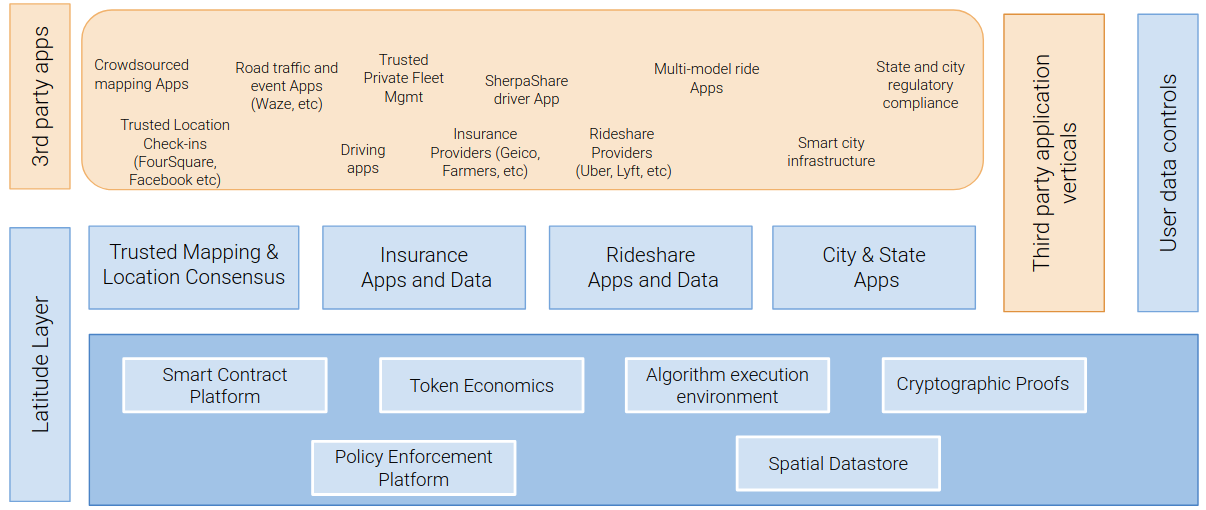
\includegraphics[width=1.00\textwidth]{latarch.png}
  \caption{Architecture of the Latitude Blockchain and associated platform ecosystem.}
    \label{fig:lat-arch}
\end{figure}

\section{The Latitude Blockchain}\label{sec:design}

In this Section, we present a high-level design of the Latitude blockchain. The full-version of this whitepaper shall
contain a very detailed design of each component. We start with an overview of the key design principles that will guide
the rest of the design for the Latitude Blockchain. Its important to note here that for implementation purposes, it
might be possible to use an existing core blockchain for the underlying functionalities and build Latitude as a layer on
top. We shall make these determinations in the full-version of the whitepaper.

The purpose of the Latitude blockchain is to become the best platform in the world for decentralized applications for
the Transportation Industry. Specifically, this boils down to constructs in the blockchain that can handle spatial,
mapping, traffic, driving data including data relating to other modalities of transport (bike sharing, walking, even air
routes later on). Figure \ref{fig:lat-arch} presents the architecture of the Latitude blockchain in terms of the core
technological innovations that will be built into it.

\subsection{Architecture overview}

The overall architecture of the Latitude Blockchain consists of a base blockchain and a side-chain for each application
vertical. This choice of an architecture gives the maximum flexibility for each side-chain to use its own mechanisms
while allowing for summaries or Merklized proofs of transactions to be commited to the base chain (or the main chain).

\begin{itemize}
    \item Overall architecture.
    \item Side chains. Main chain.
    \item chains interact mechanism.
    \item Cross-chain transactions are commitment protocol.

\end{itemize}

Each application vertical utilizes atleast one side-chain. Depending on the application, it might be necessary for
multiple side-chains to exist within a vertical, in which case we shall use composable side-chains similar to Plasma.
This allows for a hierarchical side-chain structure if needed with eventual commitment to the mainchain.

Implementation Note: For the alpha version of Latitude, it might be possible to use an existing chain with high
transaction velocity and low cost, such as EOS, Neo, Zilliqa or Harmony as a drop-in replacement for the base chain
functionality. In the long term, it might be beneficial to have our own base-chain with built in smart contract
functions for transportation applications. This will also work better with Latitude's own token economics.

\subsection{Base Blockchain layer}

Blocks, proof of stake, transaction velocity.

Delegated proof of stake system where a set of "delegates" are used. The delegates are "promoted" based on time-based
trust or stake (or a combination of these). This design is similar to the Cosmos blockchain and differs from other dPOS
system such as EOS.

The Delegated Proof of Stake (dPOS) takes the best of both cooperative and competitive consensus algorithms. DPoS uses
votes from stakeholders to achieve consensus. The competitive part is larger stakeholders having an influence on their
delegate of choice. In Latitude, it is also possible to gain a larger stake by accruing what we call "trust" through
honest operation over a period of time. The delegates that have the most votes will take their turn to produce a block
cooperatively in a sequence. DPoS is also scalable because anyone can participate in the consensus. Additionally, DPoS
is environmentally friendly because electricity isn’t wasted like in Proof of Work.

Implementation using Tendermint or plasma chains. Only Merkle proof is
committed. There can be any number of side-chains. But side-chains would correspond to one of the application platforms
described later.

PBFT for consensus on high volume side-chain commitments.

\subsection{Spatial datastore}
One of the central aspects of the Latitude blockchain is a geo-spatial datastore that fundamentally understands various
datatypes that are specific to transportation data. This datastore can use existing GIS databases that allow
de-centralized storage and access. The types of data include (i) geographic data such as location (latitude, longitude),
(ii) mapping data such as roads, terrain, addresses, etc, (iii) sensor data such as driving data, driver score, miles
driven, route information, etc, (iv) multi-modal transport data such as biking, walking and other means of transport.
Each of these data types have very special characteristics which the underlying datastore can be optimized for and allow
for programming using what we call the {\em Latitude Smart Contract} framework. 

The datastore would include spatial, quad-tree or an R-tree based indexes for efficient querying and other operations that
most Geographic Information Systems (GIS) would support in a centralized manner today. It would also include functions
to compute heatmaps, driving maps and statistics such as Traffic predictions including real-time analytics. Depending on
how Latitude evolves, the datastore can include additional functionalities to support the data sharing among autonomous
vehicles since they use most of the similar datatypes mentioned above. The datastore would support circular, rectangular
and other range queries, K-nearest neighbor searches, route optimization algorithms, etc. Figure
\ref{fig:geo_spatial_query} shows some of the queries that such a datastore can support.

%Datastore
% - Optimized for Geographic, Geo-spatial data.
% - Location, Mapping data and computation.
% - Ability to Store, index, query and build smart contracts optimized for such data.
% - Support for various spatial indexes.
% - Location heatmaps.
% - Indexing road and driving data.
% - Primitives for storing driving data for autonomous vehicles

\subsection{Cryptography layer} \label{sec:crypto} Latitude makes use of state-of-the-art cryptographic protocols to
provide various proofs, access control, confidentiality and other properties that are important in a decentralized
system.

such as AES encryption, secure hash functions, PKI certificates, multi-party key distribution protocols, proxy key
re-encryption schemes, Elliptic-curve based Digital Signatures \cite{ecdsa}. They help provide strong security, privacy,
access control, confidentiality and anonymity guarantees. Anonymity guarantees are an important part of data-sharing
smart contracts and privacy policies such as GDPR \cite{gdpr} especially for geo-spatial data such as location and maps.
Latitude provides anonymity guarantees using cryptographic set-preserving computations as derived from research in
\cite{kissner_set}. These can be suitably modified to allow for location-based anonymity which require stronger
guarantees when compared to set-based anonymity methods \cite{divanis_kanon,xu_loc_anon}.

Latitude also uses Merkle trees for cryptographic proof of audit, existence of data and verifiable computations
\cite{becker2008}. These proofs can be shared as certificates among participants or be used in the Latitude smart
contract system discussed later. They allow for verification of data existence or data-sharing contracts. They also
allow for the maintenance of a cryptographic log of all operations that happen on the network. These techniques are
similar to the ones used by some of the other blockchains today \cite{buterin_merkle}.

\subsubsection{Integrity and Access Control}

Latitude uses standard and well understood cryptographic protocols to provide robust access control and maintain basic
integrity of transactions. Data integrity is maintained using digital signatures. Every transaction is signed by one or more of the participants
certificates. The blockchain ledgers are protected using a Merkle hash \cite{becker2008} as discussed in the previous
section. A Merkle proof is used as a proof of transaction for cross-chain communication.

Access control for data that is not public or open, can be managed using multi-party key communication protocol (MPC)
\cite{enigma, nucypher, mpc_survey}. MPC protocols work over a set of $N$ trusted participants or a consortium set. They
can be designed to allow a minimum of $m<N$ participants to reach a consensus (using a off-chain protocol) in order to
compute the key that would grant access. Using these primitives, it becomes possible to have granular access control,
such as different amount of consensus for read, for writes and other semantic actions. Latitude shall make these
mechanisms available to the app developer through platform APIs. As always, since this is an open system, it is possible
for developers to build their own access control methods if they so wish.

%Cryptographic primitives for:
% - Security and privacy of data.
% - Anonymity guarantees using cryptographic set operations.
% - Enforcement of privacy when sharing data.
% - Sharing of “computation” instead of data when possible.
% - For eg: Sharing of DriverScore using a vetted algorithm.
% - Sharing proximity to a landmark instead of lat/lng.
% - Ability to find bad actors.
% - Detect privacy, anonymity and security violations.
%
%Cryptographic proofs for applications:
% - Proof of Location. 
% - Proof of ride. 
% - Proof of mapping 
%      (road/landmark exists or does not exist).
% - Proof of driver score 
% - Open, trusted, understood driver score computation algorithms.
% - Cryptographic proofs can be shared among entities, safely, securely.

In addition to these standard primitives, Latitude provides a host of other proofs that are tailor made
for geo-spatial, mapping, location and sensor data. These proofs can be used by applications, users and
other participants in the network. The network can be extended to create new forms of proofs as the application needs
grow. Below, we present the core set of cryptographic proofs that are unique to the Latitude blockchain:

\begin{figure}[t]
    \centering
    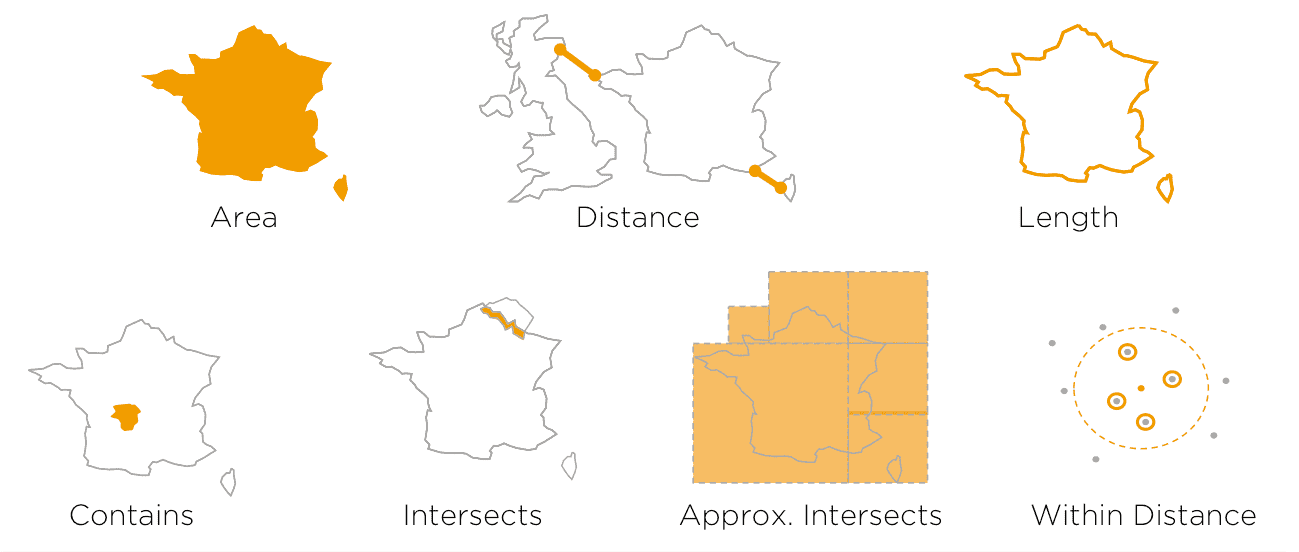
\includegraphics[width=0.70\textwidth]{geospatial_query.png}
  \caption{Examples of Geo-spatial queries that a spatial data-structure can support on the Latitude blockchain.}
    \label{fig:geo_spatial_query}
\end{figure}

\subsubsection{Proof of Real-world Observation}

A real-world observation could be a location computation, a ride from point A to B, a traffic observation or a landmark
at a given location. The core concept behind these observations is the flow of trust. The concepts presented in this
Section and the subsequent Sections replace and solve the offline Oracle problem that blockchains face today. These
mechanisms provide a practical method of creating a trust source of observation without requiring a perfect off-chain
Oracle \cite{concurrence}.

Any observation in the real world, be it a location or a landmark sighting is only as good as the trust placed in the
method and apparatus used to compute it. For example, if a GPS receiver returns a location, the amount of trust in that
location result is proportional to the amount of trust in the receiver construction and the satellite system being used
(such as Navstar, GNSS or others). Latitude uses this concept of trust as an internal metric to compute a proof of a
real-world observation.  Here we present the common algorithm used to compute these proofs which can be shared across
the Latitude platform.

\noindent
{\bf Definitions:}
\begin{itemize}
    \item Levels of trust $t_i, i \in \{0..M\}$, where $M$ is the max level of trust in the system. Trust level $t_{i+1} >
        t_i$.
    \item $t_0$ is the base level of trust assigned to any third party untrusted source of data.

    \item Each data source (such an an app installation, or a third-party source) is indentified using a certificate's
        public key. If this is a fully untrusted source that belongs to a third party, they start at the lowest level of
        trust $t_0$.

    \item $t_1$ is the trust assigned to a second party integration with Latitude's SDKs where the SDKs directly compute the
        observation and report it to the system using second-party APIs. Examples include Apps in the trusted App stores
        that integrate with Latitude.
    \item $t_2$ is the trust assigned to a first-pary integration, such as a Latitude mobile app, or a first-party app
        from trusted partners such as SherpaShare.
    \item $tmin_{pf}$ is the minimum trust needed for a specific proof or obervation. Each proof type might have a
        different requirment for this parameter. The computed proof also carries this parameters as an indication of
        consensus or trust.
    \item Trust map, $TM(e)$ gives the amount of trust recorded in the ledger for the entity $e$. The entity could be an
        organization, an individual or a user (as identified by an app installation, for example).
    \item $N_{min}$ is the minimum number of entities that need to participate in the creation of this proof. This can
        be a function of the proof being created.
    \item Concurrence Weight: Each witness that concurs with an observation provides a {\em concurrence weight} which is
        the probability that they think the event happened. This is a value between 0 and 1.
\end{itemize}

Each proof is implemented as a special smart contract supported by the Latitude platform. The smart contract that
computed these proofs would provide a signed blob of data that certifies a certain observation as determined by the
respective proof.

\noindent
{\bf Algorithm for Proof of an observation $X$}:
\begin{enumerate}
    \item Suppose $e$ is the entity that initiates a request for proof of an obervation $X$ made by $e$.
    \item The proof system finds a subset (possibly randomly sampled) of participants $S$ who are able
        to {\it concur} with the obervation $X$. Each participant, $p_i \in S$, assigns a {\em concurrence} weight
        $W(p_i, X) \in [0,1]$ depending on how well they concur with the observation.
    \item Normalization factor $Nf(p_i, X)$: This is a multiplier, usually greater than 1, that signifies the
        amplification in trust as a funciton of how the observation was concurred upon. 
    \item Each observer $p_i \in S$, provides a normalization factor $Nf(p_i, X)$ and a concurrence weight $W(p_i, X)$
        to the proof.
    \item The proof computes the total trust in the observation $X$ as $T_{pf}(X, e, S)$, given by Equation
        \ref{eq_trust_compute}.
    \item 
\end{enumerate}

\noindent
Trust computation for a proof of observation X:
\begin{equation*}
    \label{eq_trust_compute}
    T_{pf}(X, e, S) = \sum_{i\in S} T(p_i) * Nf(p_i, X) * W(p_i, X)
\end{equation*}

where $T_{pf}(X, e, S)$ is the trust for the proof of observation $X$ proposed by entity $e$ and observed by
participants $S$. A proof is considered valid if $T_{pf}(X, e, S) > tmin_{pf}(X)$, that is, the accumulated trust is
above the minimum required for the type of observation $X$.

Trust updates: Once a proof gets computed, the entity that initiated the observation gets its trust updated using an
EWMA formula. Assuming entity $e$ gets its trust updated for a proof $p_e$:
\begin{equation*}
    T(e)_{p_e} = (1 - \alpha) * T(e) + \alpha * T(p_e)
\end{equation*}

\subsubsection{Proof of Location:}

This is perhaps the most easily motivated functionality that the Latitude blockchain can provide. Proof of location is a
cryptographic credential that proves that a given user, entity or participant is/was physically present at a given
location at a specific time. The location could also be relative to another participant or landmark. The proof of
location has been explored by other blockchains such as Platin \cite{platin}. Latitude shall provide the mobile, browser
and sensor SDKs that can directly tie into the datastore to provide consensus based proofs. These proofs can unlock
applications such as access to facilities or help increase trust in crowd-sourced mapping, traffic and incident reports.

The framework provided by Latitude is general enough to capture different implementations. For instance, \cite{foam}
uses a trusted set of radio beacons or "anchors" to provide location signals. These essentially become highly trusted
observers or participants in our framework as they are essentially first-party observers (with a large amount of
base-level trust). 

\subsubsection{Proof of Ride}
\subsubsection{Proof of Landmark}
\subsubsection{Proof of DriverScore}
\subsubsection{Proof of Traffic}
\subsubsection{Proof of Route}

 \begin{itemize}
     \item Proof of location: This is perhaps the most easily motivated functionality that the Latitude blockchain can
         provide. Proof of location is a cryptographic credential that proves that a given user, entity or participant
         is/was physically present at a given location at a specific time. The location could also be relative to
         another participant or landmark. The proof of location
         has been explored by other blockchains such as Platin \cite{platin}. Latitude shall provide the mobile, browser
         and sensor SDKs that can directly tie into the datastore to provide consensus based proofs. These proofs can
         unlock applications such as access to facilities or help increase trust in crowd-sourced mapping, traffic and incident
         reports.
     \item Proof of ride: Provides a proof that a particular user has taken a ride from point A to point B using a
         certain type of transport. This proof can be used across multi-modal ride platforms such as bike or car rides.
         This can be extended to include bus trips, flights, train rides and so on. The proof of ride credential will be
         available via the Latitude mobile SDK on various platforms. Using the mobile SDK to construct these proofs also
         adds to the amount of trust on the nature and parameters of the ride.
     \item Proof of landmark (mapping): This proves the existence of a particular landmark such as a monument, a
         building, a sign post at a given lat/lng. This can also be used to prove the existence of a particular road or
         the lack of. These proofs can be constructed using the proof of location combined with consensus among users.
         This proof can become the backbone for verified mapping and landmark data-based applications.
     \item Proof of driver score: This proof can be computed on the blockchain over the data aggregated on the
         datastore. The algorithm itself shall be made available to the nodes either as an executable docker image or an
         open-source version. This allows different nodes to run the computation and create a certificate of 
         driver score which can then be attributed to the driver. This open framework can also allow different
         driver score algorithms to co-exist in the system creating a community where better driver score algorithms can
         be agreed upon and used as the industry standard.
     \item Proof of traffic:  Similar to the driver score, traffic is also an algorithm that looks at the statistics of
         location and speed data on roads. The proof is similarly computed through consensus and recorded as a
         certificate on the blockchain. The proof could be about real-time traffic or historic traffic patterns which
         can be shared with smart city applications, the Census Bureau or other regulatory bodies.
     \item Proof of routes: Similar to the functionality in the popular Waze app, this is about whether there exists a
         certain route (or a better route) from point A to point B. More the consensus, higher the trust. For example,
         if a user actually takes the route from A to B and provides a proof of ride, that helps create the proof of its existence. This is useful
         for trusted and verifiable mapping / routing applications.
 \end{itemize}

\subsection{Latitude Smart Contract system}

\begin{figure}[t]
    \centering
    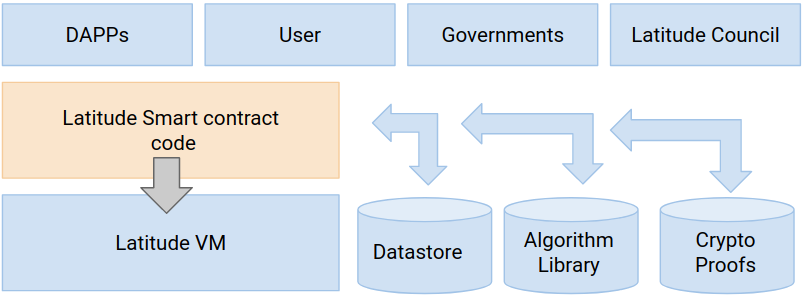
\includegraphics[width=0.60\textwidth]{lat_sc.png}
  \caption{Architecture of the Latitude Smart Contract framework.}
    \label{fig:lat-sc}
\end{figure}

Smart contracts are self-executing nuggets of code which specify the terms of the agreement between various participants
on the blockchain. For the Latitude blockchain, the participants can be a user, a regulatory body, an application
written by an insurance company or the city. The contract is directly written into lines of code in a certain smart
contract language. Popular smart contract frameworks today include ones used by Ethereum which runs on the Ethereum Virtual Machine (EVM),
the Neo which runs on the NeoVM and the EOS blockchain which runs on the WASM (WebAssembly VM).

The smart contract code and the agreements contained therein exist across the distributed, decentralized Latitude
blockchain network.  Because of this, Smart contracts permit trusted transactions and agreements to be carried out among
disparate, anonymous parties without the need for a central authority, legal system, or external enforcement mechanism.
They render transactions traceable, transparent, and irreversible as the state is always available on the Latitude
blockchain.

Figure \ref{fig:lat-sc} shows the high-level architecture of the Latitude Smart contract system. Latitude uses a
WebAssembly (wasm or eWasm) based compiler for a smart contract written in Go or C++. 

-- Overview of the webassembly architecture.

WebAssembly (or wasm) is a binary instruction format for a stack-based virtual machine. It includes a complier that is
portable and has a compilation target for high-level languages such as C++ and Go. The Latitude smart contract system
shall support both C++ and Go languages. The choice of wasm was to make the execution of the smart contract efficient
and thus have high throughput. Also, popular networks such as Ethereum are planning to move to eWasm as part of the
Ethereum Virtuam Machine (EVM) 2.0. This which will help create a common developer pool (and other aspects such as
tooling, educational material, etc) in the community. Wasm's execution happens in a safe and sandboxed
environment which can be beneficial in an adversarial and open network. It might also be possible to secure the Wasm
execution using Trusted Execution Environments (TEEs) in the near future.

The reason for chosing WebAssembly over the popular Solidity (or Vyper) used by the Ethereum Virtual Machine (EVM 1.0)
is twofold: 
WebAssembly compiles into native code and thus executes faster than Solidity or Javascript. Also, EVM 2.0 will feature
a modified version of WebAssembly, namely {\it eWasm} thus reducing the cognitive burden on developers across both
ecosystems.

Latitude uses a
modified version of Solidity (or the new Vyper programming language) as used by the Ethereum Virtual Machine. The choice
of this language is based on the production quality of the EVM, the language tools available in the community for
creating contract code, developer support and talent pool. Latitude shall add enhancements to the language to support
new spatial data types, indexes, cryptographic proofs and other mechanisms that are fundamental to the platform. Some of
the goals of the smart contract system include the ability to convert data policies such as GDPR \cite{gdpr} into
Latitude smart contract code which can then get automatically verified and enforced on the blockchain.  Also its
possible to share location data in an ephemeral manner for a specific purpose -- the data item gets automatically
destroyed using consensus and smart contract constructs on the blockchain. An example includes a user sharing their
location with an app for a very small duration of time.

As shown in Figure \ref{fig:lat-sc}, the smart contract code has access to the datastore, cryptographic proofs
(including algorithms to create proofs), an algorithm library (which hosts algorithms such as traffic, driver score
etc). These are directly accessible through language constructs making it easy to write high quality smart contract
code. The smart contract execution framework and related functionalities are accessible to dapps, entities such as
users, governments and the Latitude Council (discussed later in the Governance Section) on the system. 

The Latitude smart contract system can becomes the world's first such smart contract framework specifically tailored for
transportation data and applications.

\lstset{language=C++,basicstyle=\small}

\begin{lstlisting}[float, caption=Structure of a Latitude Smart Contract, frame=lines]

#include <latitude/contract.hpp>

// Shorthand for a location update that gets deleted in one hour.
typedef latitude::Location<TimeUnit<OneHour>> OneHourLocation;

class sample_contract : public latitude::Contract {

    private:
      // private data structures to the contract. The data does not go onchain.

    public:
      // data structures that can go onchain.
      // The contract methods will write to these.


      // There are two types of methods: Actions and callbacks.

      void onLocationUpdate(latitude::OneHourLocation curr) {
          // business logic
      }

      void computeProximity(OneHourLocation given, Location<NoExpiry> target) {
          // business logic
      }
}
\end{lstlisting}

\begin{itemize}

    \item Explain action methods.
    \item Data structures.
    \item Callback methods.
    \item Events.

\end{itemize}

\subsubsection{Secret contracts}

Typical smart contracts are public, including the data they operate on. For privacy or other reasons, it might be
desirable to achieve consensus on data without making it open on the chain. Latitude supports what are called secret
contracts using multi-party key distribution protocols. Multi-party key distribution creates a set of keys, such that a
function (or a smart contract) can be computed in a distributed manner over a random piece of data without any single
entity having full access to the data. The result of the computation has consensus and can be put on-chain using a
cyrptographic proof or can be directly communicated to a decentralized  app.

The availability of Trusted Execution Environments or hardware enclave can dramatically assist in the implementation of
secret contracts. In the first version of Latitude, we shall use existing MPC communication protocols in this area to
create a secret contract system similar to the one used in Enigma \cite{enigma}. In a later version, it might become
possible to use TEEs using a design similar to Ekiden \cite{ekiden}.

% Smart contract system for Transportation
% applications.  - Ability to convert “policies” such as GDPR into smart contract code.  - Example, self destruct data
% after a time period.  - Sandboxed trusted execution environment: - For algorithms: - DriverScore, Location heatmaps,
% Statistics.  - Enforcing or verifying privacy and other govt policies/regulations.


\subsubsection{Contract sharding}

Latitude smart contracts will be sharded to improve performance. Existing blockchains such as Ethereum, Neo and EOS
suffer from slow throughput on smart contract execution. One technique that has recently emerged as a way to scale
performance is to shard the contract using annonatations on methods to expose specific semantics. For example, by
understanding portions of a smart contract that store data, that verify computations and that are callbacks from
user-facing apps, it becomes possible to separate the execution among parallel nodes for much higher throughput
\cite{chainspace}. 

For example, in a given smart contract, certain data structures are annotated to store data. The dependencies between
the data structures is also specified as a group. There are three kinds of methods: Actions, callbacks and Verifiers. 
The Callbacks are used by the system to update the contract when a data or event happens, such as a user updates their
location. The Action methods are executed by the smart contract to take an action and the verifiers are methods that
verify transaction state. By isolating these methods and their data dependencies, one can shard a smart contract to
execute in pieces on different nodes on a blockchain thereby increasing efficiency and reducing the probability of a
coordinated attack.

Much like the other components, Latitude's smart contract sharding system shall leverage available algorithm libraries
and tools for rapid and iterative development.

\subsection{Token economics: The Latitude Token (LAT)}

Latitude has its own token for use on the Latitude Blockchain, called LAT. There would be a fixed token supply for a
certain period of time (4 years). A certain percentage of the tokens are reserved for funding and other operations, the
detials of which are not discussed in this document. The rest of the tokens will be available for the network for use.

{\bf INSERT TOKEN PIE CHART}
\newline
\noindent
{\bf Cryptoeconomics:}
Cryptoeconomics refers to the mechanics of the protocol underlying the blockchain operations which creates incentives
for the various stake-holders. For example, in the Latitude Blockchain it is possible to reward users for sharing their data
for certain purposes. For example, users can be rewarded if they share traffic data or accident information or better
routes. This is similar to the Waze model but creates legitimate rewards for users that have meaningful value outside
the Waze application. For an overview of Cryptoeconomics in the blockchain space, please see \cite{sinclair_crypto}.

The core building block of the Cryptoeconomics in Latitude is the Latitude Token, or LAT. This will be transacted in
each and every micro-transaction that takes place on the blockchain to create the right incentives, enforce smart
contracts and penalize Byzantine behavior. One of the fundamental design principles behind the protocol for the LAT
token is to create incentives assuming nodes are greedy and are interested in maximizing their gain. We will also build
safeguards against reasonable amount of collusion among nodes to subvert the system. The design is crafted such that the
best way for a node to maximize its revenue would be to participate with full honesty.

Latitude shall employ a Proof of Stake model (delegated or non-delegated) for participation and core node-level mining. This mechanism has recently
gained popularity among a notable number of blockchains \cite{dpos_steemit}. This also allows for deposit slashing as a
technique to tackle Byzantine behavior. Latitude will employ techniques such as Minimal Slashing \cite{buterin_slashing}
for Byzantine fault tolerance and safety under distributed asynchronous operation.

\noindent
{\bf User incentives:}
Token economics allow for the creation of what we call user incentives. These are protocol constructs in the blockchain
that allow users to benefit from the value they create for the ecosystem. Refer to \cite{token_ecos} for an overview on
incentive mechanisms to reward users for various methods of participation in the network. In general, the Latitude token
ecosystem will be based on market economics, that is, supply and demand from various participants will be the primary
driver for prices and incentives in the network. This philosophy falls in line with decentralized control and operation
while also allowing for creating most reward for honest behavior in the network.

The ability of user incentives to exist in a decentralized manner can be disruptive to existing incumbents in the
sharing economy space, such as Uber, Lyft, Airbnb, etc since users can get rewarded in a tangible manner for their
contributions \cite{sharing_eco_bc}. Consumers shifted to apps in the sharing economy as they provided cheaper and
better alternatives to traditional services like Uber and Airbnb. However, since all transactions go through these
centralized providers, the platform owners determine the fees, percentages and are in complete control of any data
practices and policies which cannot be verified. They often become accused of predatory behavior. Using blockchain based
incentives, sharing and open-source software these problems can be addressed in a singular fashion.

As an example, consider the Ridesharing application. As users contribute data on what rides they are taking, it becomes
possible for the network to reward them with tokens. They could, upon sufficient contribution, redeem them for free
rides or share with them others on the network. A similar model can be adopted for data concerning driver behavior where
drivers using different apps and sensor algorithms can elect to share their data towards building a better driver score
in return for suitable incentives.

\subsection{Governance on Latitude}

Governance refers to a decentralized manner in which decisions are made using a consensus mechanism on the blockchain.
Decisions include basic constructs whether a node can join or leave the network. Or it can include key decisions on
whether an upgrade should be mandated on every node, a given participant such as a data provider should be penalized. It
could also include issues where humans get involved, such as when a user complains of a loss of privacy or a breach in
contract.

Recently blockchains have been moving towards governance using a small set of participants, such as trusted miners in
the case of Stellar and Ripple \cite{stellar_gateway}. The EOS blockchain uses a similar concept of a core set of block
producers who are elected based on a nomination and voting process \cite{eos_producers}. For discussion around
Governance in Ethereum, refer to \cite{buterin_gov}. Latitude uses a similar concept of a {\em council} of participants.
These are entities (nodes or organizations) that have demonstrated participating using earned trust through honest
operation, accumulating stake, demonstrated good intent and establishing trust. Some members of this council might
include the core Latitude developers which allows them to implement operations such as updates, bug fixes and so on. The
council members shall be elected using the an election protocol on the blockchain. It might be possible to directly
nominate certain council members such as regulatory bodies who have general interest in user rights, privacy and
enforcement. 

% - Crypto-incentives for honest operation.
% - Penalties for malicious intent.
% - Governance based on consensus and roles using a council.
% - Council members elected using voting, stake and established trust.
% - Some council members can have restricted access.
% - Eg: US govt can have voting rights on US data/users, etc.
%

\begin{figure}[t]
    \centering
    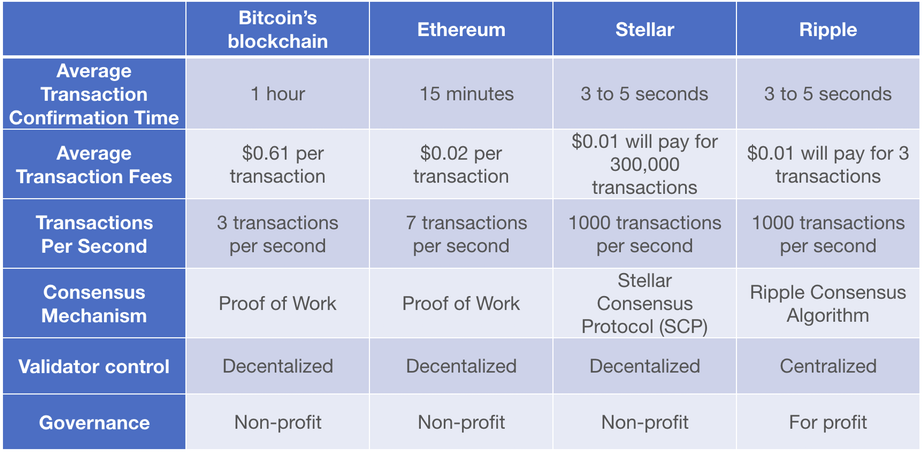
\includegraphics[width=0.90\textwidth]{tps_speed2.png}
  \caption{Comparison of transactions per second of the major blockchains today.}
    \label{fig:tps_speed}
\end{figure}

\subsection{Performance considerations}
When thinking of performance, one of the key metrics that is hotly debated in the community is transactions per second.
Bitcoin is know for its long time to produce a block, on the order of minutes which limits the number of transactions
the network can process. Figure \ref{fig:tps_speed} shows a comparison of the major blockchains today with respect to
this crucial metric. Note that these blockchains shown in the Figure are primarily evaluated against the concept of a
transaction which represents a transfer of assets, goods or monetary value digitally on the blockchain. Stellar and
Ripple are two blockchains that have gained popularity for financial transactions as they tout a higher transaction
velocity. 

In the context of Latitude, the performance of the blockchain is important. The blockchain will handle different types
of data and transactions which will require different levels of consensus and trust. Figure \ref{fig:tps_lat} shows the
different types of transactions that the Latitude blockchain can process and the performance we expect to achieve. Shown
are four types of transactions:
\begin{itemize}
    \item Datastore transactions: These refer to basic transactions to store data values into the geo-spatial data
        store. For instance, if a user shares their driving data, this can include the sensor information, lat/lng of
        the trip taken and any mapping data collected. For ride-sharing applications, this can include any multi-model
        ride details that the user has booked. We expect the blockchain to be able to process close to 1-10 million
        transactions per second, since most such transactions require very low level of consensus and can tolerate 
        eventual consistency \cite{eventual_con}.
    \item Algorithmic computations: These refer to transactions which include executing known algorithms on the
        blockchain. For instance, this could include the computation of various driver behavior algorithms with the
        computation being shared among certain participants on the network. Another computation could include statistics
        such as real-time traffic or aggregate traffic statistics shared with a city for better zoning and planning
        purposes. The amount of consensus required is relatively small but higher than datastore operations in order to
        ensure correct execution of algorithms and lack of malicious intent. Also such operations would require strong
        consistency for their CRUD functionalities. We expect the Latitude design to support 10-100K transactions per
        second at its peak usage.
    \item Data sharing contracts: These transactions refer to the creation, deletion or arbitration of long-term sharing
        smart contracts between participating entities. For instance, it could include a new contract between an
        insurance company and a data provider for sharing certain types of driver score data for certain geographic
        locations. Since these transactions have higher value they require larger amount of trust and consensus in the
        system. Latitude shall support a transaction speed of around 100-1000 transactions per second for this category.
    \item Governance operations: The Governance operations require the highest amount of trust and full consensus of the
        network. These include voting to add/remove council members, critical council decisions such as forks or
        updates/upgrades, decisions on high-value smart contract disputes, etc. The transaction velocity is low for
        reasons of trust, accuracy and correctness and thus we expect the Latitude blockchain to support 1-10
        transactions per second under this category.

\end{itemize}

Another metric of importance for Latitude is the storage capacity in the network. This can be important for
datastore operations. We expect the storage capacity, network bandwidth and any other computing resource to become
available on an incentivized model as determined by usage contracts. For instance, if a user is willing to share data with
a data consumer, the consumer should be able to allocate token resources to provision the network with sufficient
storage. The token can be used to purchase storage using other blockchain storage providers such as Filecoin, Siacoin or
Golem can be used to incentivized nodes to directly supplant on-chain storage.

\begin{figure}[t]
    \centering
    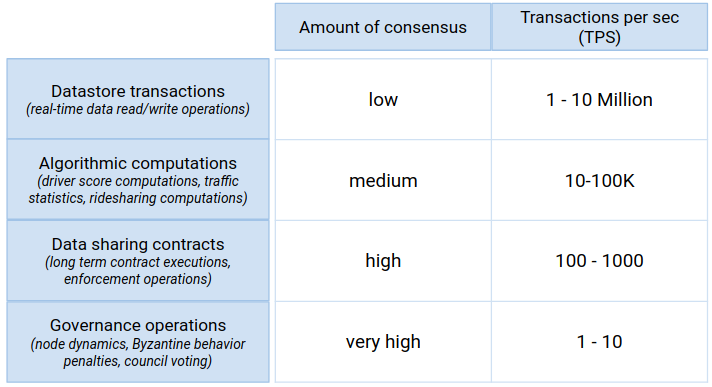
\includegraphics[width=0.75\textwidth]{tps_lat2.png}
  \caption{Expected Transaction per second velocity of various types of functionalities on the Latitude Blockchain.}
    \label{fig:tps_lat}
\end{figure}

